\documentclass[12pt,letterpaper]{article}
\usepackage[utf8]{inputenc}
\usepackage[spanish]{babel}
\usepackage{graphicx}
\usepackage[left=2cm,right=2cm,top=2cm,bottom=2cm]{geometry}
\usepackage{graphicx} % figuras
% \usepackage{subfigure} % subfiguras
\usepackage{float} % para usar [H]
\usepackage{amsmath}
%\usepackage{txfonts}
\usepackage{stackrel} 
\usepackage{multirow}
\usepackage{enumerate} % enumerados
\renewcommand{\labelitemi}{$-$}
\renewcommand{\labelitemii}{$\cdot$}
% \author{}
% \title{Caratula}
\begin{document}

% Fancy Header and Footer
% \usepackage{fancyhdr}
% \pagestyle{fancy}
% \cfoot{}
% \rfoot{\thepage}
%

% \usepackage[hidelinks]{hyperref} % CREA HYPERVINCULOS EN INDICE

% \author{}
\title{Caratula}

\begin{titlepage}
\begin{center}
\large{UNIVERSIDAD PRIVADA DE TACNA}\\
\vspace*{-0.025in}
\begin{figure}[htb]
\begin{center}

\includegraphics[width=8cm]{./Imagenes/logo}
\end{center}
\end{figure}
\vspace*{0.15in}
INGENIERIA DE SISTEMAS  \\

\vspace*{0.5in}
\begin{large}
TITULO:\\
\end{large}

\vspace*{0.1in}
\begin{Large}
\textbf{INFORME DE LABORATORIO No 01} \\
\end{Large}

\vspace*{0.3in}
\begin{Large}
\textbf{CURSO:} \\
\end{Large}

\vspace*{0.1in}
\begin{large}
INTELIGENCIA DE NEGOCIOS\\
\end{large}

\vspace*{0.3in}
\begin{Large}
\textbf{DOCENTE(ING):} \\
\end{Large}

\vspace*{0.1in}
\begin{large}
 Patrick Cuadros Quiroga\\
\end{large}

\vspace*{0.2in}
\vspace*{0.1in}
\begin{large}
Integrantes: \\
\begin{flushleft}


Mamani Ayala  Brandon \hfill  (2015052715) \\
Ordoñez Quilli Ronald 	\hfill  (2015052821) \\
Quispe Mamani Angelo        \hfill	(2015052826) \\
Rodriguez Mamani Juan        \hfill	(2017057862) \\
Vizcarra Llanque Jhordy        \hfill	(2015052719) \\
\end{flushleft}
\end{large}
\end{center}

\end{titlepage}


\tableofcontents % INDICE
\thispagestyle{empty} % INDICE SIN NUMERO
\newpage
\setcounter{page}{1} % REINICIAR CONTADOR DE PAGINAS DESPUES DEL INDICE

\section{Actividad No 01 – Manipulaci\'on de Datos} 

\begin{enumerate}[1.]
	\item El departamento de Recursos Humanos requiere crear sentencias SQL para insertar, actualizar y eliminar datos de empleados. Como prueba se utilizará la tabla Mis\_Empleados antes de remitir las sentencias al departamento de Recursos Humanos.

	\item Crear la tabla Mis\_Empleados utilizando la siguiente estructura.
	\begin{center}
	\includegraphics[width=8cm]{./Imagenes/imagen0102} 
	\end{center}
	\item Generar una sentencia de inserción de datos que permita añadir los siguientes registros:
	\begin{center}
	\includegraphics[width=8cm]{./Imagenes/imagen0103} 
	\end{center}

	\item Generar un script que permita que mediante utilización de variables de sustitución, la inserción de información en la tabla Mis\_Empleados.

	\item Utilizando el script anterior adicionar los siguientes registros.
	\begin{center}
	\includegraphics[width=5cm]{./Imagenes/imagen0105} 
	\end{center}
	\item Revisar los cambios hechos a la tabla.
	\item Cambiar el nombre del empleado No 3 a Benjamín.
	\item Elevar el salario a \$ 1,000 a todos los empleados que tengan un salario menor a esa cantidad.
	\item Eliminar el registro del empleado María Castro
	\item Revisar los cambios hechos a la tabla.
	\item Confirmar los cambios a la tabla.
	\item Adicionar el siguiente registro a la tabla
	\\exec insertar\_datos 6,'Hurtado Gamboa','Ernesto','ehurtado',1400
	\\ go
	\item Revisar la adición realizada
	\item Crear un punto de restauración intermedio para esta transacción
	\item Borrar los registros de la tabla MIS\_EMPLEADOS.
	\item Revisar los cambios realizados.
	\item Descartar los cambios hechos a la tabla sin descartar la última adición hecha.
	\item Revisar nuevamente los registros de la tabla MIS\_EMPLEADOS.
	\item Confirmar todos los cambios hechos a la tabla MIS\_EMPLEADOS.
	\item Modificar el script del punto 4.4. a fin de que se genere automáticamente el CODIGO del empleado que lo conforman la primera letra de su nombre y la primera palabra de su apellido.
	\item Adicionar el siguiente registro a la tabla a fin de corroborar el funcionamiento del script anterior
           \\exec insertar\_datos 7,'Valdivia Pérez','Graciela',1800;
           \\go
	\item Revisar los cambios realizados. Y finalmente confirmar todos los cambios hechos a la tabla MIS\_EMPLEADOS.
\end{enumerate}  	 	
\section{INTRODUCCION} 

En los \'ultimos años, las organizaciones han recurrido cada vez mas a soluciones de software avanzadas para administrar las cargas de trabajo, mantener la rentabilidad y asegurar la competitividad dentro de sus respectivas industrias. Si bien hay varias opciones disponibles, las herramientas de inteligencia de negocios (BI) y las herramientas de an\'alisis de negocios (BA) son posiblemente las soluciones de administraci\'on de datos mas implementadas. Los analistas de negocios y los compradores de software a menudo preguntan cuáles son las diferencias clave entre la inteligencia de negocios y los análisis de negocios.

Las soluciones de inteligencia empresarial se encuentran entre las herramientas de administraci\'on de datos mas valiosas disponibles. Las soluciones de BI recopilan y analizan datos actuales y procesables con el fin de proporcionar información para mejorar las operaciones comerciales. ¿Est\'a buscando formas de entender mejor sus operaciones comerciales? ¿Qu\'e hay de descubrir puntos de dolor en sus flujos de trabajo? ¿Qu\'e hay de analizar grandes conjuntos de datos para obtener información valiosa? Necesita una solución de inteligencia de negocios.

El software de an\'alisis de negocios es un niño o padre (dependiendo de a qui\'en le pregunte) de la categor\'ia de inteligencia empresarial. Al igual que BI, se utiliza principalmente para analizar datos hist\'oricos, pero con la intención de predecir las tendencias de negocios. Por lo general, también tiene un ojo hacia la mejora y la preparación para el cambio.
\section{MARCO TEORICO} 
		
\begin{enumerate}[1.]
	\item Business Analytics :
\\
\\
Al igual que la inteligencia de negocios, BA recopila y analiza datos, emplea análisis predictivos y genera informes visualizados en paneles personalizados. El objetivo de estas características es ayudar a identificar y abordar los puntos débiles de una organización. Aquí es donde terminan las similitudes. El software de análisis de negocios se utiliza para explorar y analizar datos históricos y actuales. Utiliza el análisis estadístico, la extracción de datos y el análisis cuantitativo para identificar las tendencias comerciales anteriores.
\\
Una vez que se han recopilado y analizado los datos, los sistemas de análisis de inteligencia empresarial los utilizan para el modelado predictivo. Esto puede predecir y, en la mayoría de los casos, prepararse para futuros climas empresariales. Uno de los aspectos más poderosos de BA es el informe ad-hoc, que permite a las empresas realizar análisis de datos específicos en tiempo real para responder preguntas específicas para tomar decisiones comerciales más rápidas. En efecto, el análisis de negocios utiliza el análisis predictivo para resolver problemas antes de que hayan ocurrido.

\end{enumerate}

\begin{center}
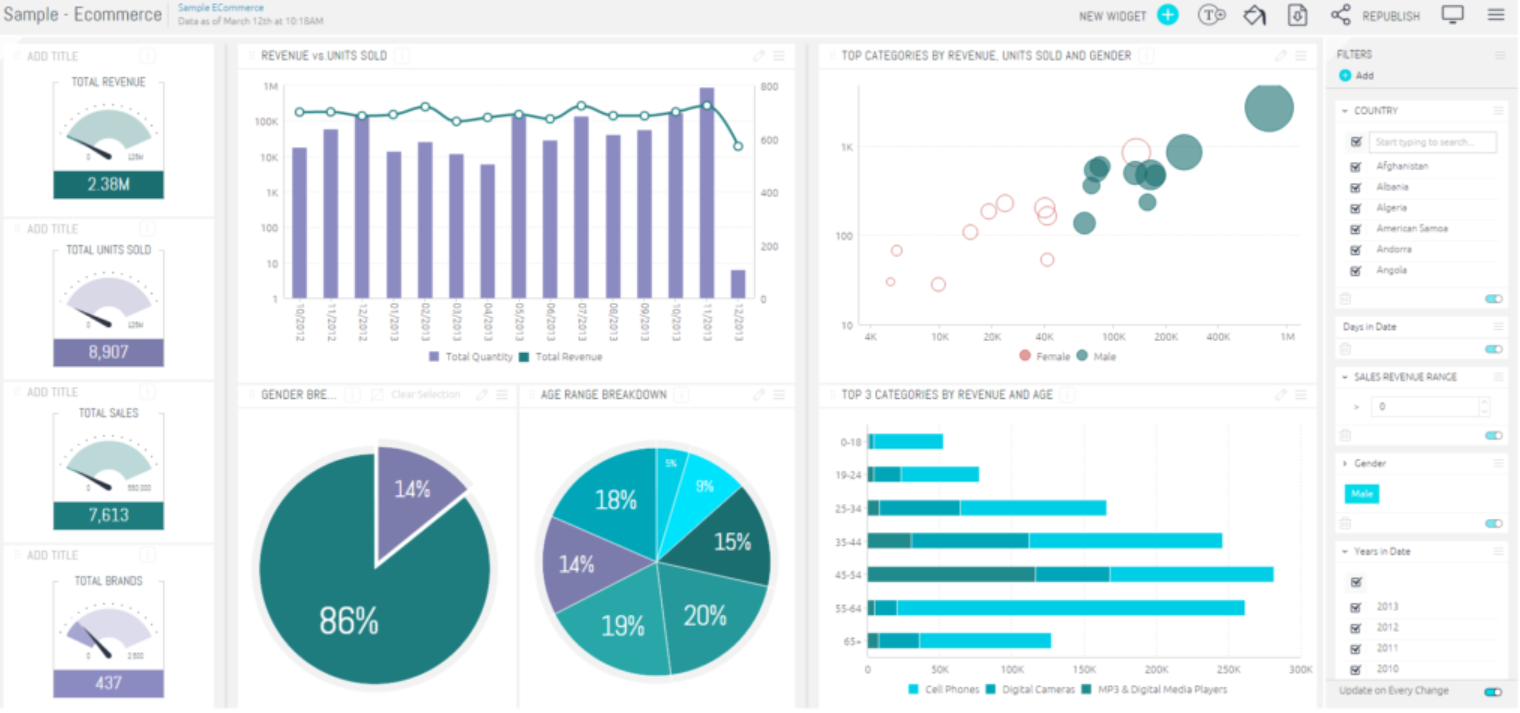
\includegraphics[scale=0.55]{./Imagenes/BA.png}
\end{center}


\section{APLICACION} 
		
\begin{enumerate}[1.]

	\item Aplicaciones BI :
\\
\\
 Una de las claras tendencias en el mercado Business Intelligence es la mayor importancia que los clientes otorgan a visualizar la informaci\'on de una manera sencilla, \'agil y potente. Todo a la vez.
\\
\\
- La entrega de informaci\'on contin\'ua siendo el foco central de la mayor\'ia de los proyectos de BI en la actualidad, pero vemos una creciente demanda de herramientas que permitan un an\'alisis más fácil e intuitivo para descubrir nuevas perspectivas. (Gartner, 2010)
\\
\\
-Pr\'oxima generaci\'on de aplicaciones de Business Intelligence pretenden ir más all\'a de la provisi\'on de informaci\'n en gr\'aficos circulares y estad\'isticos, para proporcionar representaciones m\'as visuales e intuitivas de datos y tendencias. (IDG)
\\
\\
- Herramientas como la visualizaci\'on de datos (en formatos que van m\'as all\'a de las simples im\'agenes est\'aticas) permiten presentar informaci\'on de forma clara y eficaz. La visualizaci\'on de datos ha estado directamente relacionada con las tecnolog\'ias de BI desde su origen y la b\'usqueda continuada de presentaciones m\'as eficaces e interactivas a trav\'es de la visualizaci\'on ser\'a uno de los objetivos de las soluciones anal\'iticas de los pr\'oximos años. (Federico Navarro Cabrera, de IBM)
\\
\\
Hasta hace muy poco, el Business Intelligence era una manera m\'as o menos sencilla de generar informes, listados, an\'alisis, o "reportes"(¡que horrible palabra!)... Al final, todo era m\'as o menos lo mismo... Informes tabulares, con filas y columnas llenas de n\'umeros, y alg\'un gr\'afico. Las herramientas m\'as avanzadas permit\'ian añadir alertas semaf\'oricas, parametrizar el informe, o alg\'un tipo de navegaci\'on OLAP (que raramente se utilizaba)... Este tipo de soluciones ya han llegado a su madurez, y existe muy poca diferencia entre la oferta de los diferentes proveedores..
\\
Sin embargo, esta manera tradicional de acceder a la informaci\'on resulta insuficiente (e ineficiente), y cada vez m\'as las organizaciones buscan maneras de proporcionar a sus usuarios soluciones para acceder, analizar y comprender la informaci\'on corporativa de una manera m\'as sencilla, din\'amica, visual e intuitiva. El cambio es realmente profundo, y supone una renovaci\'on completa en las "interfases de usuario"...
\\
Estoy hablando de soluciones tipo QlikView, Tableau o, por supuesto, Bingo Intelligence... que buscan la mayor usabilidad para el usuario final, y ofrecen soluciones Business Intelligence muy interactivas y visuales... Os dejo algunos pantallazos de Qlickview y Tableau.

\end{enumerate}

\begin{center}
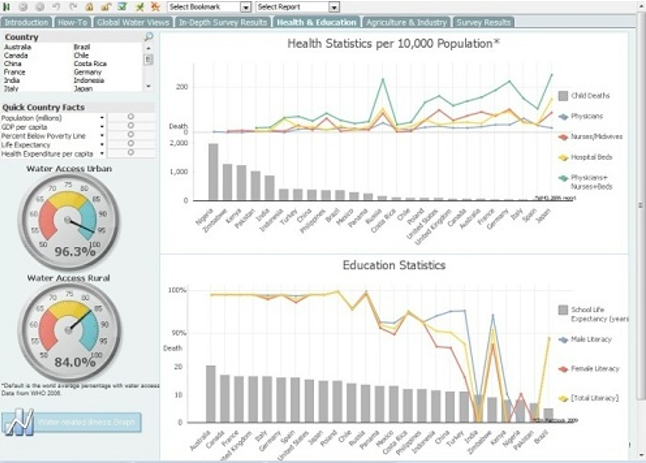
\includegraphics[scale=0.60]{./Imagenes/img1.png}
\end{center}

\begin{center}
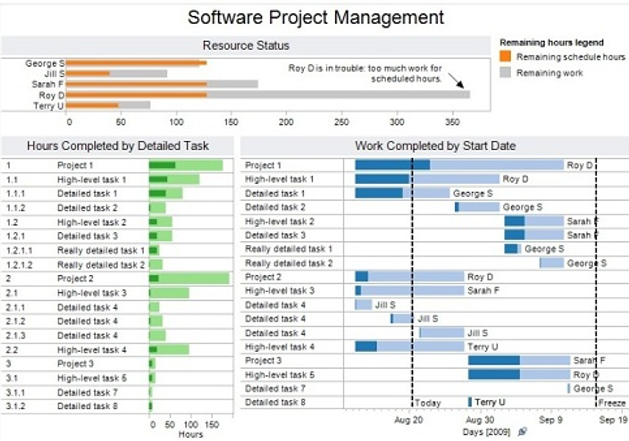
\includegraphics[scale=0.60]{./Imagenes/img2.png}
\end{center}

\begin{center}
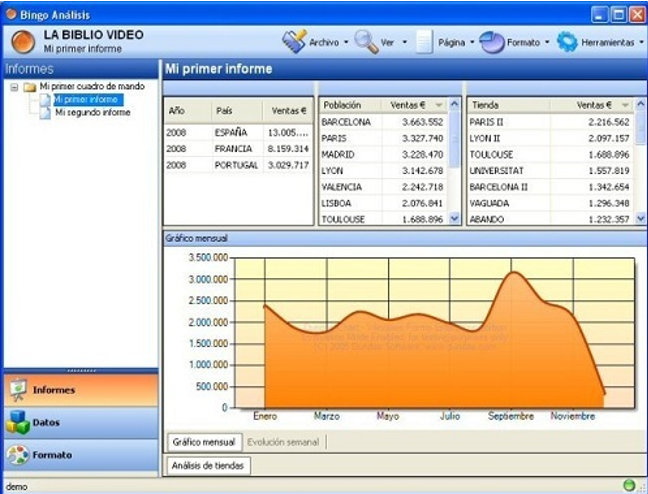
\includegraphics[scale=0.60]{./Imagenes/img3.png}
\end{center}

\begin{center}
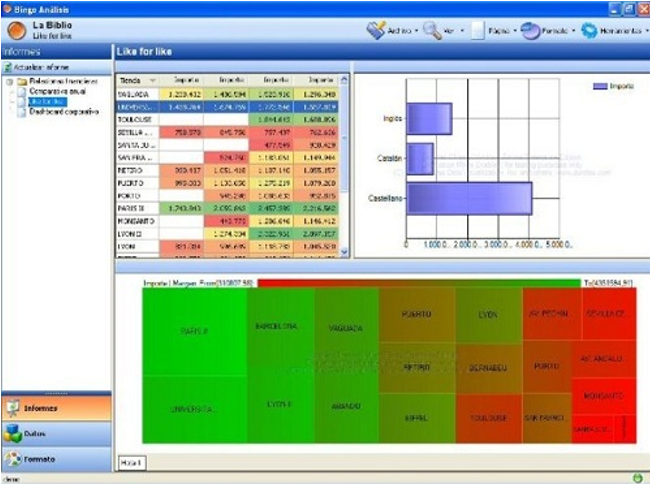
\includegraphics[scale=0.60]{./Imagenes/img4.png}
\end{center}

\begin{enumerate}[2.]

	\item Aplicaciones BA :
\\
\\
Empecemos con un ejemplo de su aplicaci\'on una cafeter\'ia quiere elegir la ubicaci\'on de un nuevo local en Lima. Antes de tomar esta decisi\'on tienen que estar muy seguros sobre la ubicaci\'on de este, porque una vez creado el local, revertir la situaci\'on seria muy costoso. Los usuarios de internet podr\'ian proporcionar informaci\'on sobre su lugar de residencia y sobre posibles locaciones en las cuales les gustar\'ia que el local este ubicado para poder asistir, tambi\'en se puede encontrar informaci\'on de zonas en las que no est\'e presente una empresa de este rubro para poder abarcarla. Lo que hace BA, es recuperar toda esta informaci\'on para ayudar a la empresa a definir sus planes y poder explicar el porqué de la elecci\'on de su nueva locaci\'on. Confiar en este tipo de datos que proporciona BA reduce el riesgo de tomar una decisi\'on desinformada y err\'onea.
\\
\\
Enfocado al marketing podemos decir que las empresas usan el BA para sacar ventaja a la competencia, ya que se anticipan a las nuevas necesidades de cliente. Se pueden relevar nuevas tendencias de consumo o uso de los productos con el uso del BA.
\\
\\
El poder de transformaci\'on de los datos es realmente grande, sin embargo, el poder no est\'a en los datos por s\'i solo, sino tambi\'en a medida que se pulen a trav\'es de an\'alisis. Aunque la anal\'itica se ha convertido en parte de un lenguaje diario, definimos el BA como el proceso de descubrimiento de conocimiento para la acci\'on y la creaci\'on de nuevas oportunidades de negocio a partir de esos descubrimientos. La lecci\'on principal es ligar fuertemente en BA a los negocios. Para ello, se tiene que crear intersecciones seguras y productivas con el personal que se encarga del análisis y los decisores estrat\'egicos.


\end{enumerate}


\section{CONCLUSIONES} 
		
\begin{enumerate}[1.]
	\item El Departamento de Recursos Humanos requiere ocultar ciertos datos de la tabla EMPLOYEES, Ellos necesitan una vista llamada VW\_Empleados, que contenga los campos ID del Empleado, Nombres e ID del Departamento.
	\item Utilizando la vista anterior crear un reporte que muestre los nombres y departamentos a los cuales
pertenecen los empleados.
	\item El departamento 50 requiere acceso a los datos de los empleados. Generar una vista llamada VW\_Dept50, que contenga las columnas ID del Empleado, Apellidos e ID del Departamento de los empleados del departamento 50. Etiquetar las columnas como EmpNo, Empleado y DeptNo. Por razones de seguridad no se debe permitir a los empleados ser reasignados a otros departamentos.
	\item Probar la vista, tratando de reasignar al empleado Matos al departamento 80.
	\item Se requiere crear una secuencia que será utilizada en la Llave Primaria de la tabla Departamentos (tabla creada en la práctica anterior). La secuencia deberá iniciar con el valor 200 y terminar en el valor 1000, asimismo deberá incrementarse en 10 cada vez que se requiera. Nombrar la secuencia SEQ\_Departamentos\_ID.
	\item Para probar la secuencia, adicionar dos registros a la tabla Departamentos, Educación y Administración. Verificar la adición.
	\item Crear un índice no único en la columna NOMBRE de la tabla Departamentos.
	\item Crear un sinónimo para la tabla EMPLOYEES con el nombre EMP.
\end{enumerate}


\section{REFERENCIAS} 
		
\begin{enumerate}[1.]
	
\begin{thebibliography}
\textbf{[1]} Julio Castro. ¿Qué es la inteligencia de negocios y cómo beneficia a tu empresa?. 2015 https://blog.corponet.com.mx/que-es-la-inteligencia-de-negocios\\\\

\textbf{[2]} Samuel Esteban. Consejos para hacer crecer tu negocio. 2015 https://es.workmeter.com/blog/bid/177356/qu-es-el-business-intelligence\\\\

\textbf{[3]} Database Hardening Best Practices. https://prezi.com/htejn8bxdiwd/aplicacion-de-inteligencia-de-negocios\\\\

\textbf{[4]} Michel Frank Tello Alegria. Aplicacion de la inteligencia de negocios. 2018 https://www.businessintelligence.info/mercado/software-business-intelligence-visual-e-intuitivo.html\\\\

\textbf{[5]} 
Medina. Business Intelligence. una guía práctica. 2012 https://editorial.upc.edu.pe/publicaciones/business-intelligence-una-guia-practica-2da-edicion\\\\

\textbf{[6]} Webmining. Business Analytics versus Business Intelligence. 2012 http://www.webmining.cl/2012/03/business-analytics-versus-business-intelligence\\\\


\end{thebibliography}


\end{enumerate}



\end{document}
